\section{Learning the Pareto-optimal Set Efficiently }
\label{sec:learn-pareto-optim}

In this section, we discuss techniques that learns the Pareto-optimal set
efficiently. We first describe our programming abstraction and profiling
formalism. We then focus on addressing two challenges: $(i)$ We propose to use
Bayesian Optimization (BO) to address large parameter space with multiple
parameters. And we show that it outperforms previous approaches (random search
and coordinate search). $(ii)$ We propose to use profile transfer to derive the
profile for a new device without running expensive profiling from scratch.

\subsection{Programming Abstraction for Compute Adaptation}
\label{sec:progr-abstr}

Unlike \autoref{sec:structure-adapt}, the algorithms and parameters do not come
from a series of chained operators. Therefore, we need new programming
abstractions here. However, the design goal is similar: to free developers from
specifying exact rules and allow specifications with options.

We use \texttt{trait}\footnote{\texttt{trait} in Rust is similar to
  \texttt{interface} in other languages.} to abstract each algorithm, as below:

\begin{lstlisting}[xleftmargin=.1\textwidth, xrightmargin=.1\textwidth, language=Rust]
trait Algorithm {
    type I;
    type O; 
    type P;
    fn execute(&mut self, i: &Self::I, p: &Self::P) -> Self::O;
}
\end{lstlisting}

Each algorithm is specified by its input data type \texttt{I}, output data type
\texttt{O}, a parameter type \texttt{P}, and its behavior function
\texttt{execute}. For any data type \texttt{T} that implements
\texttt{Algorithm} trait, the function \texttt{execute} can access the internal
data structure of \texttt{T} in a mutable way: \texttt{\&mut self}. Type
\texttt{I}, \texttt{O}, and \texttt{P} are abstract types and the implementation
must specify the concrete types. We show an implementation of Viola-Jones in
\autoref{fig:vj} where the input type is an image, the output type is a
detection, and the parameter is \texttt{VJParameters}.

For tunable parameters, we need to be able to specify at least three parts:
\texttt{min}, \texttt{max}, and \texttt{step}. We extend an algorithm's
parameter by augmenting it with annotations. In Rust, this can be implemented
with procedural macros as a syntax extension. \autoref{fig:vj} shows these
annotation in blue: we use \texttt{\#[derive(Adapt)]} to mark that this
\texttt{struct} is a tunable parameter and use \texttt{\#[adapt(...)]} to mark
its field.

\begin{figure}
  \centering
\begin{lstlisting}[language=Rust]
#[derive(Adapt)]
struct VJParameters {
    #[adapt(min = "0", max = "20", step = "1")]
    min_neighbors: i64,

    #[adapt(min = "0", max = "190", step = "10")]
    min_size: i64,

    #[adapt(min = "1.01", max = "1.5", step = "0.01")]
    scale_factor: f64,
}

impl Algorithm for VJ {
    type I = Image;
    type O = Detection;
    type P = VJParameters;

    fn execute(&mut self, image: &Image, opt: &VJParameters) -> Detection {
        // ...
    }
}
\end{lstlisting}
  \caption{Viola-Jone face detector parameters annotated with adaptation (in
    Rust).}
  \label{fig:vj}
\end{figure}

\subsection{Profiling Formalism}
\label{sec:profiling-formalism}

We assume there are multiple algorithms $\mathbb{A}$ available to provide the
same inference. For each algorithm $a \in \mathbb{A}$, it has parameters tunable
to affect processing time $t$ and inference accuracy (or utility $u$). These
parameters could be related to data, such as lowering the image resolution, or
related to the algorithm, such as increasing the scaling factor in HOG. One
instance of the parameters forms a configuration
$\vec{c} = (k_1, k_2, \dots, k_n)$ with $n$ dimensions---we explicitly use the
arrow head here to emphasize configurations' high dimensionality. Running the
algorithm $a$ with a configuration $\vec{c}$ on a machine $m$ yields an
inference with utility $u$ and processing time $t$.

We denote this performance model as a mapping:

that is, for any configuration $c$ in the Pareto-optimal set $\mathbb{P}$, there
is no alternative configuration $c'$ that requires less processing times (i.e.,
$T(c') < T(c)$) and offers a higher accuracy (i.e., $A(c') > A(c)$). Formally,
$\mathbb{P}$ is defined as follows:

{\small \vspace{-1em}
  \begin{equation*}
    f: (\mathbb{A} \times \mathbb{P} \times \mathbb{M}) \rightarrow
    (\mathbb{R}\times \mathbb{R})
\end{equation*}
} where $\mathbb{A}$ is the set of all algorithms, $\mathbb{C}$ is the set of
all possible configurations, and $\mathbb{M}$ is the set of all machines. The
mapping returns two real values: execution time $t \in \mathbb{R}$ and utility
$u \in \mathbb{R}$. For convenience, we use $\vec{x}$ for the tuple $(a, c, m)$.
Also we use $f_t$ and $f_u$ for the mapping from variables to time $t$ and
utility $u$, respectively.

Bounding the response times is trivial if application accuracy can be
arbitrarily low. \sysname{} aims to minimize response times while maximizing
achievable accuracy---solving a multi-objective optimization problem,
specifically two objectives. For these problems in general, there is no single
optimal solution that jointly minimizes multiple objectives. Instead, there is a
collection of optimal solutions where for any solution, no objective can be
improved without damaging one of the other objectives. The goal of our
performance modeling is to derive such Pareto-optimal
set~\cite{collette2013multiobjective} across all possible
configurations. Formally, the Pareto-optimal set is defined as follows,

{\small \vspace{-1.2em}
  \begin{equation}
    \mathbb{P} = \{ c \in \mathbb{C} : \{ c' \in \mathbb{C}: T(c') < T(c),
    A(c') > A(c) \} = \varnothing\}
  \label{eq:pareto-2}
\end{equation}
\vspace{-1.2em}
}

\para{Challenge.} The Pareto-optimal set is easy if we know the mapping for all
possible arguments. However, in practice, the argument space is prohibitively
large, especially for configurations $\vec{c}$ that have many tunable
parameters. It is expensive to run all combinations. Besides, it is also
impossible because developers may not have target machines available.

\para{Solution Overview.} We tackle each dimension differently. For algorithms,
because their differences are substantial, our profiler evaluates all available
algorithms exhaustively. For each algorithm, to address the curse of
dimensionality of $\vec{c}$, we use BO to reduce space search and only find
near-optimal $c$s. For different machine $m$, because only $f_t$ depends on $p$,
we show that the Pareto-optimal set doesn't change if the execution time $f_t$
satisfies monotonicity. We approximate $f_t$ with a simple linear model.

\subsection{Composing Algorithms}
\label{sec:compose-models}

There are different algorithms. Different implementation for GPU and CPU.

We have to profile each individual algorithm.

Observation: their profile (the Pareto-optimal set) are composable by merge and
compare all of them.

\subsection{Modeling Parameters}
\label{sec:single-platform}

Evaluating all configurations across the large parameter space is prohibitively
expensive. To reduce the number of samples we need, we build a performance model
that is just accurate enough to allow us to distinguish near-optimal
configurations from the rest. This is similar to recent systems, such as
CherryPick~\cite{alipourfard2017cherrypick} and BOAT~\cite{dalibard2017boat},
that use Bayesian optimization (BO) to improve performance across a large number
of configurations.

While previous approaches often transform the multi-objective problem into a
single-objective problem using scalarization techniques (an approach that is
expected to be suboptimal~\cite{knowles2006parego}.) We adopted the
PESMO~\cite{hernandez2016predictive}, which does not transform the
multi-objective problem into a single-objective. PESMO also has a low
computational cost. It grows linearly with respective to the total number of
objectives $K$.

\subsubsection{Introduction to Bayesian Optimization}
\label{sec:bo}

Bayesian optimization approximate black-box functions with proxy functions and
iteratively proposes new sample point in the large parameter space. Effective
for,

\begin{itemize}
\item Evaluating each sample is expensive.
\item The objective is a black-box.
\item The evaluation can be noisy
\end{itemize}

Gaining attraction beyond ML scope. CherryPick~\cite{alipourfard2017cherrypick}
finds the best cloud configurations for big data analytics. Google optimize
chocolate chip cookies recipes~\cite{solnik2017bayesian}.

Acquisition function evaluates the utility of candidate points for the next
evaluation of $f$, balancing a high objective (exploitation) and high
uncertainty (exploration)~\cite{shahriari2016taking}.

Expected Improvement "ei"

Figure produced with mlrMBO package~\cite{bischl2017mlrmbo} based on Alpine N. 2
function~\cite{clerc1999swarm}.

Maximum is 7.92 with a value of 2.808119.

\begin{figure}
  \begin{subfigure}{\textwidth}
    \centering
    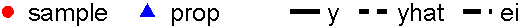
\includegraphics[width=0.5\textwidth]{figures/bo-legend.pdf}
  \end{subfigure}
  \vspace{0.2em}
  \\
  \centering
  \begin{subfigure}{0.45\textwidth}
    \centering
    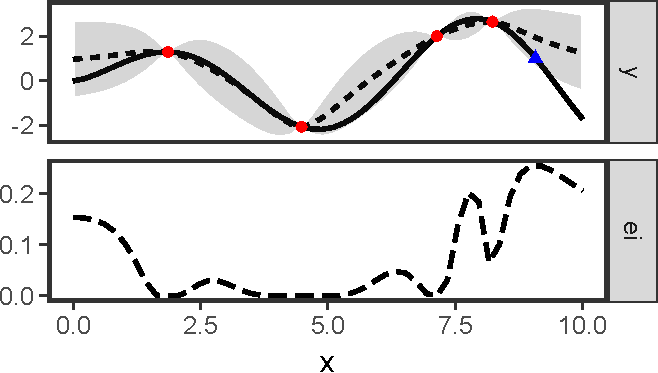
\includegraphics[width=\textwidth]{figures/bo1.pdf}
    \caption{First Iteration.}
  \end{subfigure}
  \hspace{1em}
  \begin{subfigure}{0.45\textwidth}
    \centering
    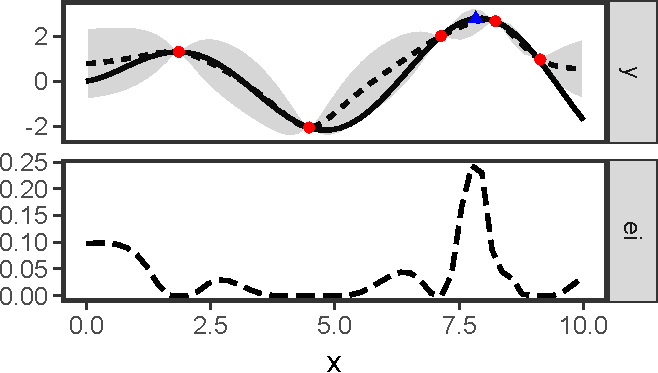
\includegraphics[width=\textwidth]{figures/bo2.pdf}
    \caption{Second Iteration.}
  \end{subfigure}
  \caption{Bayesian Optimization illustrated.}
  \label{fig:bo-1d}
\end{figure}

\begin{figure}
  \centering
  \begin{subfigure}{0.45\textwidth}
    \begin{tikzpicture}
      \pgfplotstableread{
        0 0.1 -0.1
        0 0.1  0.2
        1 0.25 0.5
        2 0.4  0.6
        3 0.5  0.85
        4 0.9  0.9
        4 1.2  0.9
      }\datatable
      \begin{axis}[
        width  = \textwidth,
        xlabel = Processing Times (normalized),
        ylabel = Accuracy,
        axis line style = thick,
        ymin   = 0,
        ymax   = 1,
        ytick  = {0, 0.2, 0.4, 0.6, 0.8, 1},
        xmin   = 0,
        xmax   = 1,
        xtick  = {0, 0.2, 0.4, 0.6, 0.8, 1},
        ]

        \addplot+[red!50,
        mark size=3pt, mark options={draw=red!0, fill=red!80}, const
        plot mark left, thick] table [x index=1, y index=2]{\datatable};

        \addplot[mark=triangle*, mark options={draw=blue!80, fill=blue!80},
        mark size=3pt, fill=blue!80, only marks]
        coordinates { (0.3, 0.7) };

        \draw[-, blue, dashed] (axis cs:0.3, 0.5) -- (axis cs:0.3, 0.7);
        \draw[-, blue, dashed] (axis cs:0.3, 0.7) -- (axis cs:0.5, 0.7);
        \draw[<->, >=stealth, blue] (axis cs:0.45, 0.6) -- (axis cs:0.45, 0.7);
        \draw[<->, >=stealth, blue] (axis cs:0.3, 0.55) -- (axis cs:0.4, 0.55);

      \end{axis}
    \end{tikzpicture}
  \end{subfigure}
  \hspace{1em}
  \begin{subfigure}{0.45\textwidth}
    \begin{tikzpicture}[
      triangle/.style = {fill=blue!80, regular polygon, regular polygon sides=3}
      ]

      \pgfplotstableread{
        0 0.1 -0.1
        0 0.1  0.2
        1 0.25 0.5
        2 0.4  0.6
        3 0.5  0.85
        4 0.9  0.9
        4 1.2  0.9
      }\datatable
      \begin{axis}[
        width  = \textwidth,
        xlabel = Processing Times (normalized),
        ylabel = Accuracy,
        axis line style = thick,
        ymin   = 0,
        ymax   = 1,
        ytick  = {0, 0.2, 0.4, 0.6, 0.8, 1},
        xmin   = 0,
        xmax   = 1,
        xtick  = {0, 0.2, 0.4, 0.6, 0.8, 1},
        axis on top
        ]

        \addplot+[blue!50, no marks,
        mark size=3pt, mark options={draw=blue!0, fill=blue!80},
        % pattern=north east lines,
        % pattern color=blue!50,
        fill=blue!20,
        ]
        coordinates {(0.3, 0.5) (0.3, 0.7) (0.5, 0.7) (0.5, 0.6) (0.4, 0.6)
          (0.4, 0.5) (0.3, 0.5)};

        \addplot+[red!50, mark=*,
        mark size=3pt, mark options={draw=red!0, fill=red!80}, const
        plot mark left, thick,
        pattern=north west lines,
        pattern color=red!50]
        table [x index=1, y
        index=2]{\datatable} \closedcycle;

        \addplot[mark=triangle*, mark options={draw=blue!80, fill=blue!80},
        mark size=3pt, fill=blue!80, only marks]
        coordinates { (0.3, 0.7) };
        
      \end{axis}
    \end{tikzpicture}
  \end{subfigure}
  \caption{Comparison of additive-epsilon (left, arrows) and hypervolume (right,
    filled areas) improvements for two possible new observations (green and
    blue) to the current Pareto front (red points). The reference point for
    hypervolume computations is the black crossed circle.  In terms of epsilon
    improvement, the green point is more interesting as it is farther away from
    the Pareto front, but the blue point is better in terms of volume
    increment.}
\end{figure}

We use PESMO~\cite{hernandez2016predictive} and compare it with two baselines:
(1) greedy/coordinate search; (2) random search. PESMO chooses evaluation points
to maximally reduce the entropy of the posterior distribution over the Pareto
set.


\subsection{Modeling Machines}
\label{sec:performance-transfer}

We make the observation that $f_u(a, c, m)$ doesn't depend on $m$. If we assume
a monitonicity between $f_t(m_1)$ and $f_t(m_2)$, we can prove that the
Pareto-set is directly transferable. The monitonicity is a condition that if on
one platform it takes longer for one configuration,
i.e.\,$f_t(a, \vec{c}, m_1) < f_t(a, \vec{c'}, m_1)$, then it will take longer
on another platform, i.e.\,$f_t(a, \vec{c}, m_2) < f_t(a, \vec{c'}, m_2)$.

Based on these two assumption, one can prove that if $\vec{x}_i$ is in the
Pareto-optimal set $\mathbb{P}_1$ for platform $p_1$, then $\vec{x}_i$ will also
be in the Pareto-optimal set $\mathbb{P}_2$. And the profile on $p_2$ will be a
stretched or shrunk version for $p_1$ along the time dimension.

This simplifies our model transfer across platforms and makes it possible to
derive the performance model at runtime by sampling only a few performance
measures. In practice, a simple linear transformation suffices in giving a
reasonably precise transfer.

%%% Local Variables:
%%% mode: latex
%%% TeX-master: "../compute"
%%% End:
